%%------------------------------------------------------------------------------
%%Präambel laden
%%------------------------------------------------------------------------------
%%------------------------------------------------------------------------------
%%Klasse
%%------------------------------------------------------------------------------
\documentclass[a4paper,DIV=calc,11pt,titlepage]{scrartcl}
%%------------------------------------------------------------------------------
%%Packages
%%------------------------------------------------------------------------------
\usepackage[headsepline=0.5pt, footsepline=0.5pt]{scrlayer-scrpage}
\usepackage{scrdate}
\usepackage[utf8]{inputenc}
%\usepackage{lmodern}
\usepackage{CJKutf8} 				
\usepackage[ngerman]{babel} 
\usepackage{geometry}
\usepackage[colorlinks=true,linkcolor=Navy,pdfborder={0 0 0},pdftex,pdfauthor={Sascha Christmann},pdftitle={G\={o}j\={u}-Ry\={u} Karate-D\={o} Reusrath - Trainigskompendium},pdfproducer={MiKTeX},pdfcreator={pdflatex},pdfsubject={Prüfungsinhalte - Erwartungshorizont - Ergänzungen}]{hyperref}
\usepackage{tabularx}
\usepackage[svgnames,RGB,table]{xcolor}					
\usepackage{booktabs} 						
\usepackage{multicol,multirow}
\usepackage{caption}
\usepackage[oldstyle]{libertinus}			%Schriftart -> Libertine, Minuskeln
%\usepackage[sfdefault]{noto}				%Schriftart -> Noto Sans, -> Schriftgröße auf 10pt runter!
\usepackage[T1]{fontenc} 							
\usepackage[german]{layout}
\usepackage{textcomp}
\usepackage{calc}
\usepackage{microtype}
\usepackage{float}
\usepackage{tikz}
\usepackage{tcolorbox}
\usepackage{layout}
\usepackage{graphicx}
\usepackage{amssymb}
\usepackage{amsmath}
\usepackage{mwe}
%%------------------------------------------------------------------------------
%%Vereinbarungen & Makros
%%------------------------------------------------------------------------------
\clearpairofpagestyles
\setlength{\footskip}{23pt}
\setlength{\textheight}{721pt}
\setlength{\textwidth}{451pt}
\setlength{\headheight}{42pt}
\setlength{\marginparsep}{0pt}
\setlength{\marginparwidth}{72pt}
\setlength{\topmargin}{-47pt}
\setlength{\oddsidemargin}{0pt}
\pagestyle{scrheadings}
\setkomafont{pagehead}{\normalsize} 
\setkomafont{pagefoot}{\footnotesize}			%setzt Kopfzeile auf nicht kursiv
\addtokomafont{caption}{\color{Gray}}
\renewcommand*{\sectionmarkformat}{}		% Kapitelnummerierung in der Kopfzeile aus → KOMA-Script-Anleitung
\automark[section]{section}
\cfoot{\pagemark}
\newcounter{num}
\newcounter{numz}
\newcommand{\ctu}[0]{\stepcounter{num}\arabic{num}.}
\newcommand{\ctuz}[0]{\stepcounter{numz}\arabic{numz}}
\newcommand{\ctd}[0]{\addtocounter{num}{-1}\arabic{num}.}
\newcommand{\ctdz}[0]{\addtocounter{numz}{-1}\arabic{numz}}	
\setcounter{num}{0}
\setcounter{numz}{0}


\newlength\tindent
\setlength{\tindent}{\parindent}
\setlength{\parindent}{0pt}
\renewcommand{\indent}{\hspace*{\tindent}}

\newlength{\VTe}
\settowidth{\VTe}{\tiny Zuki, Age-Uke, Yoko-Uke, Harai-Otoshi-Uke, Soto-Uke, Uraken-Uchi, Empi-Age-Uchi, Mae-Geri, Mawashi-Geri}

\graphicspath{{Gfx/gkd/}{Gfx/habersetzer/}{Gfx/}{Gfx/div/}{Gfx/espeloer_heckhuis_kata/}{Gfx/gurte/}{Gfx/sglgrkr/}{Gfx/tartaglia/}{Gfx/unsuidojo/},{Gfx/wolfskehlen/},{Gfx/self/}{Gfx/yuishinkan_kamen/}}

\definecolor{GKD}{rgb}{0.53,0.086,0.102}
\definecolor{SGL}{rgb}{0,0.580,0.290}
\definecolor{SGL2}{rgb}{0,1,0}

\let\svthefootnote\thefootnote
\newcommand\freefootnote[1]{%
	\let\thefootnote\relax%
	\footnotetext{#1}%
	\let\thefootnote\svthefootnote%
}

\newenvironment{KANJI}{%
	\CJKfamily{ipxm}%
	\CJKtilde
	\CJKnospace}{}
%%------------------------------------------------------------------------------
%%EOF
%%------------------------------------------------------------------------------
%%------------------------------------------------------------------------------
%%Ende Präambel
%%------------------------------------------------------------------------------
\begin{document}
	\layout
	%%------------------------------------------------------------------------------
%%ToDo
%%------------------------------------------------------------------------------
%%	
%%	Copyright nachpflegen
%%	\captionlistentry[figure]{Logo \textcopyright\, \href{https://www.sglangenfeld.de/de/wettkampf/karate-goju-ryu-reusrath/}{G\={o}j\={u}-Ry\={u} Karate-D\={o} Langenfeld Reusrath}}
%%	\captionlistentry[figure]{Netzfundstück G\={o}j\={u}-Ry\={u} Karate-D\={o} Kanji Schriftzeichen}
%%	Gürtel-SVG von https://upload.wikimedia.org/wikipedia/commons/7/76/Judo_black_belt.svg
%%	Oder Gürtel TBD: https://creativecommons.org/licenses/by-sa/4.0/deed.en
%%	https://commons.wikimedia.org/wiki/File:Karate_white_belt.svg
%%	https://commons.wikimedia.org/wiki/File:Karate_yellow_belt.svg
%%	https://commons.wikimedia.org/wiki/File:Karate_orange_belt.svg
%%	https://commons.wikimedia.org/wiki/File:Karate_green_belt.svg
%%	https://commons.wikimedia.org/wiki/File:Karate_blue_belt.svg
%%	https://commons.wikimedia.org/wiki/File:Karate_brown_belt.svg
%%	https://commons.wikimedia.org/wiki/File:Karate_black_belt_2.svg
%%	
%%------------------------------------------------------------------------------
%%ToDo
%%------------------------------------------------------------------------------
	%%------------------------------------------------------------------------------
%%SOF Titel
%%------------------------------------------------------------------------------
	\title{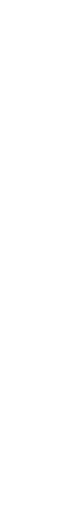
\includegraphics[height=10cm]{GJR_kanji_placeholder_left}\quad
\includegraphics[height=10cm, keepaspectratio=true]{GJRKDR_n}\quad
\includegraphics[height=10cm]{GJR_kanji}\rmfamily\\Prüfungsanforderung\\Erwartungshorizont\\Ergänzung}
	\author{\sffamily Sascha Christmann\and\sffamily Powered by \rmfamily\LaTeX 2$_{\varepsilon}$}
	\subtitle{9. Kyu - Shodan\\Ausarbeitung zum 1. Dan}
	\begin{titlepage}
		\maketitle
	\end{titlepage}
%%------------------------------------------------------------------------------
%%EOF
%%------------------------------------------------------------------------------

	\tableofcontents\newpage
	\begin{figure}
		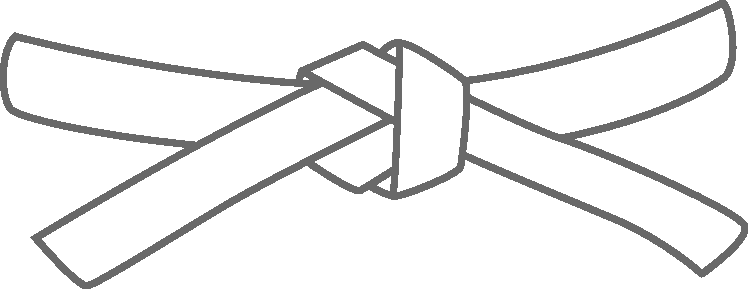
\includegraphics[width=.12\linewidth]{weissgurt}\hfill
		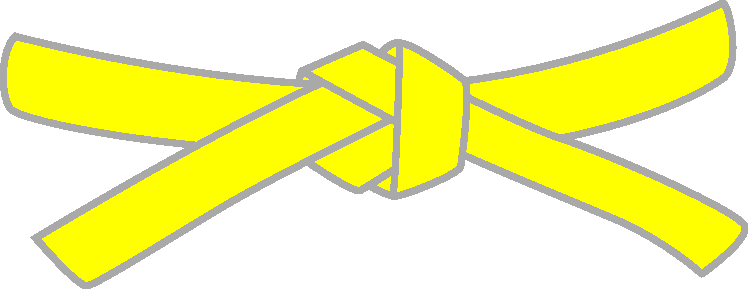
\includegraphics[width=.12\linewidth]{gelbgurt}\hfill
		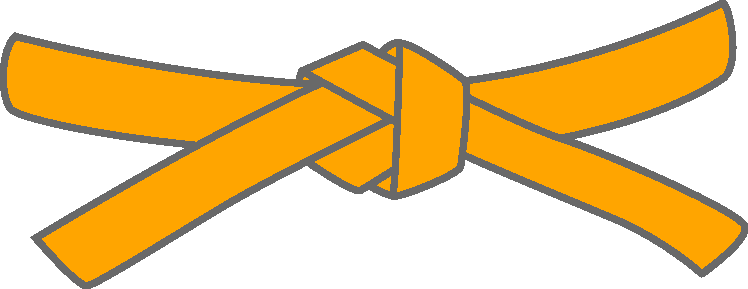
\includegraphics[width=.12\linewidth]{orangegurt}\hfill
		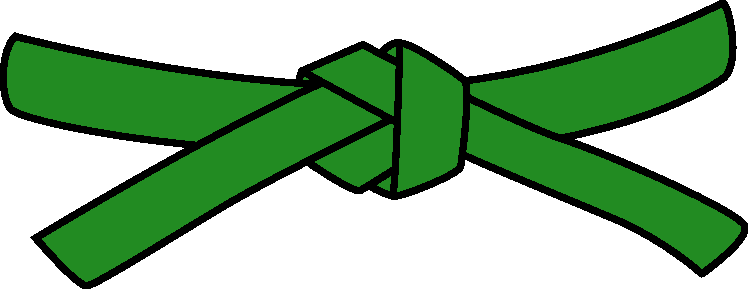
\includegraphics[width=.12\linewidth]{gruengurt}\hfill
		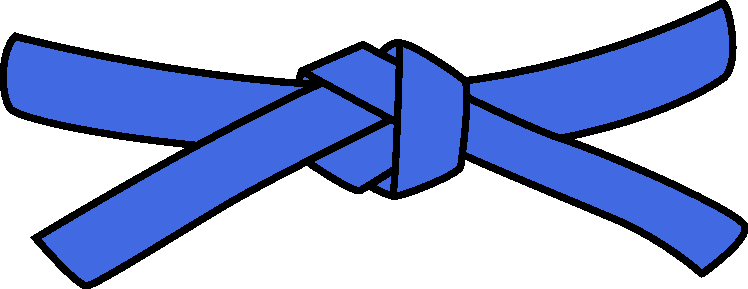
\includegraphics[width=.12\linewidth]{blaugurt}\hfill
		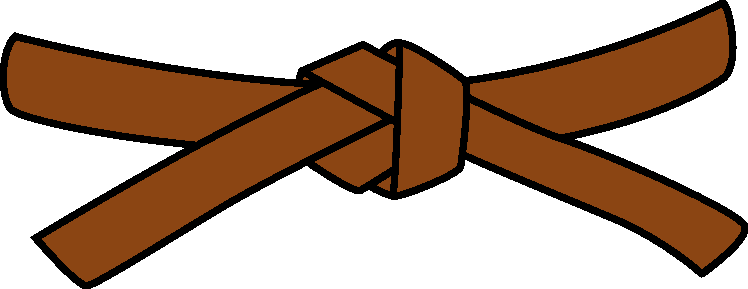
\includegraphics[width=.12\linewidth]{braungurt}\hfill
		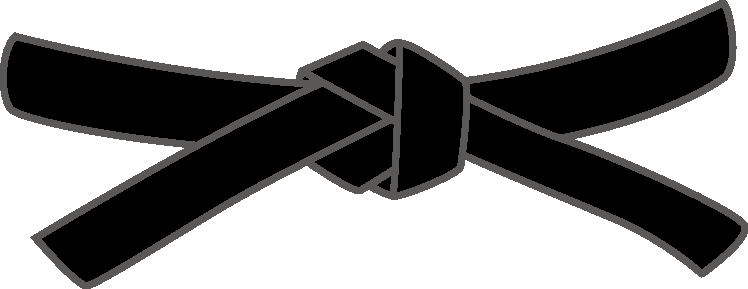
\includegraphics[width=.12\linewidth]{schwarzgurt}\\
		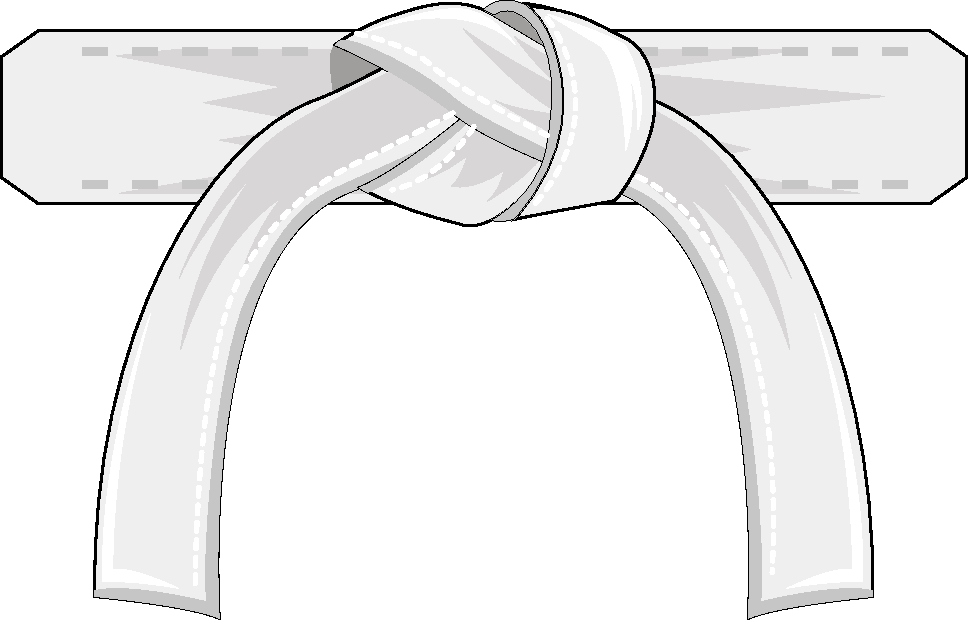
\includegraphics[width=.12\linewidth]{whitebelt}\hfill
		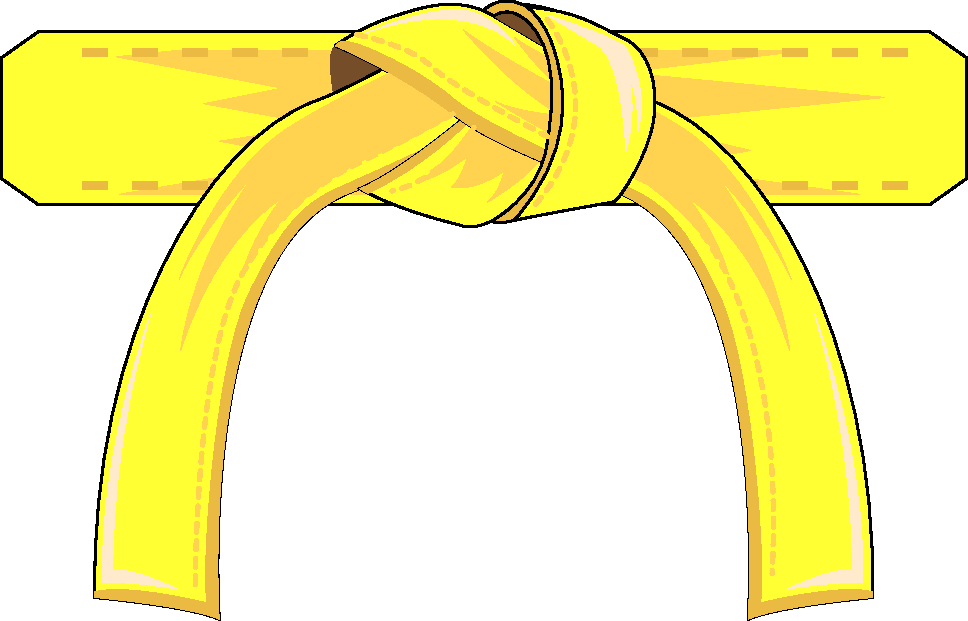
\includegraphics[width=.12\linewidth]{yellowbelt}\hfill
		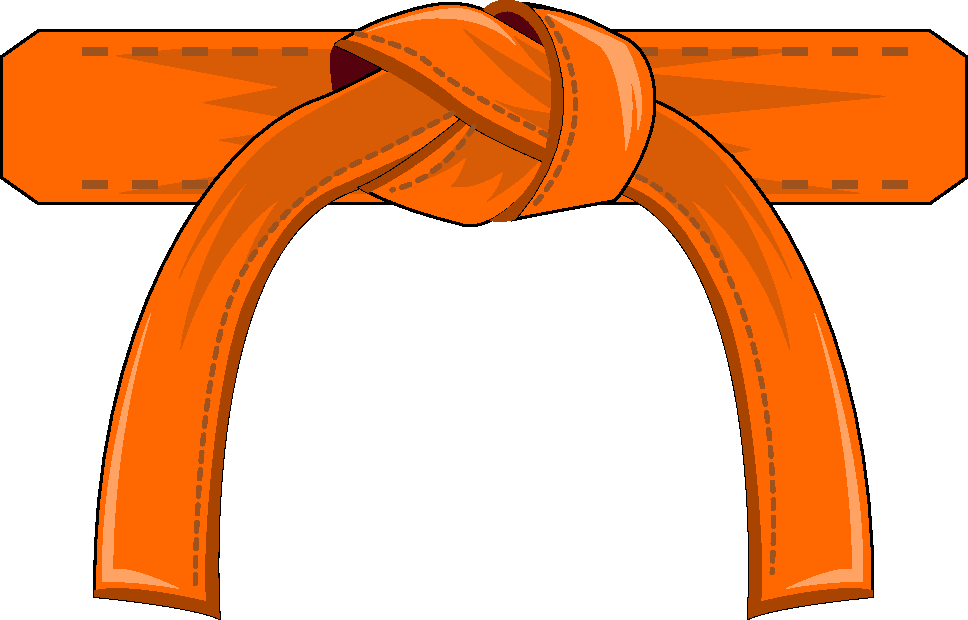
\includegraphics[width=.12\linewidth]{orangebelt}\hfill
		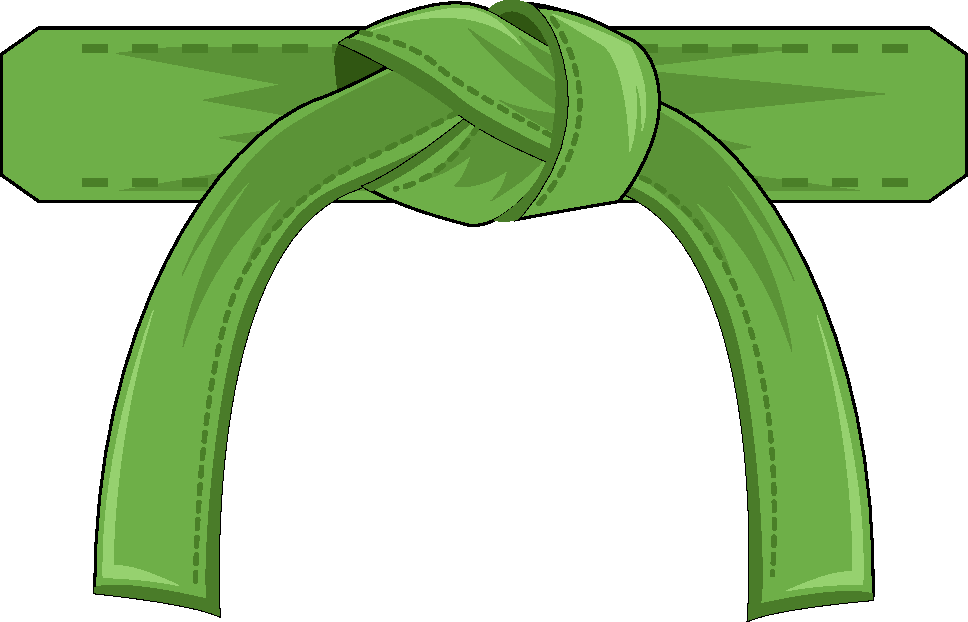
\includegraphics[width=.12\linewidth]{greenbelt}\hfill
		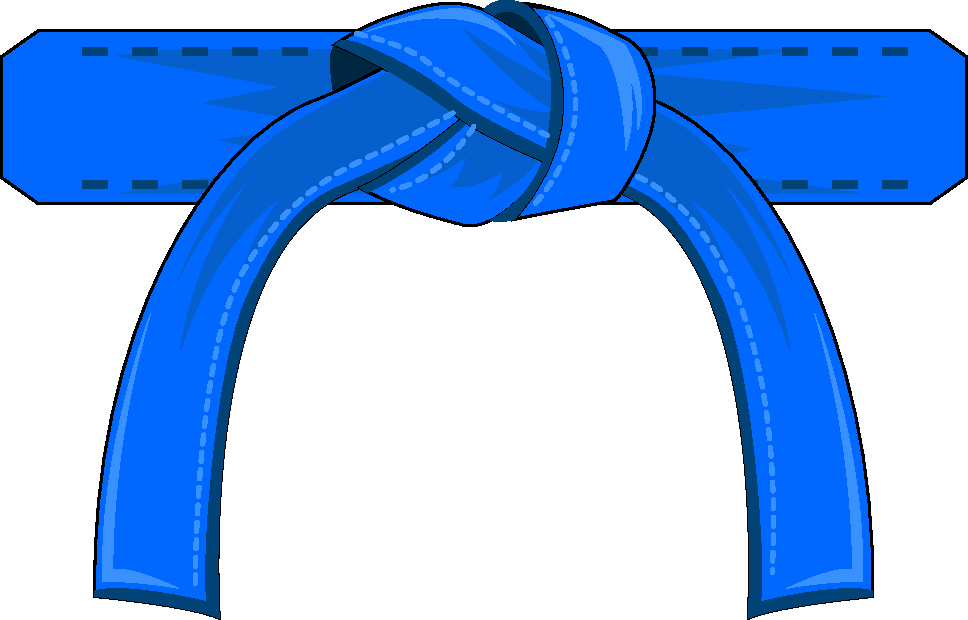
\includegraphics[width=.12\linewidth]{bluebelt}\hfill
		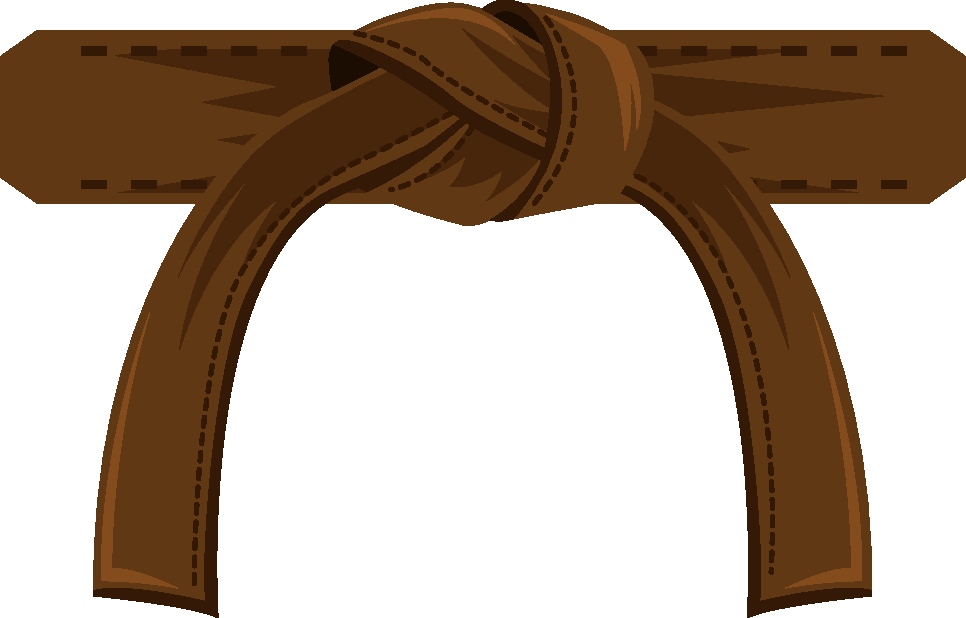
\includegraphics[width=.12\linewidth]{brownbelt}\hfill
		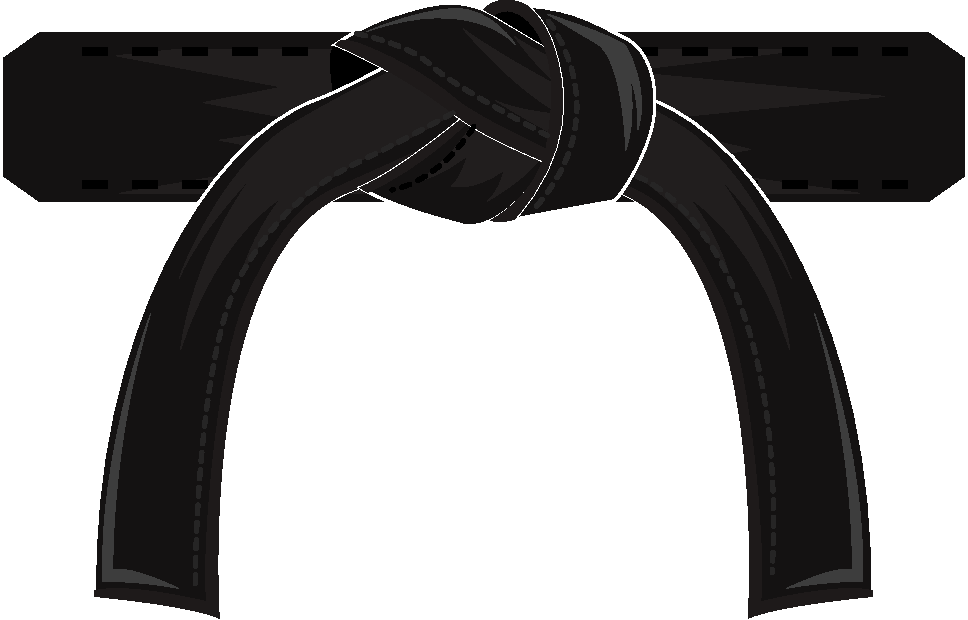
\includegraphics[width=.12\linewidth]{blackbelt}\\
		\caption{MWE to demonstrate how to place to images side-by-side}
	\end{figure}
	\clearpage
	%%------------------------------------------------------------------------------
%%Allgemeines
%%------------------------------------------------------------------------------
	\setcounter{num}{0}
	\setcounter{numz}{0}
	\begin{tcolorbox}[width=\textwidth,right=12pt,left=12pt,colframe=lightgray,colback=white,fonttitle=\bfseries,coltitle=black,title=Allgemeines:\indent Trainingsablauf Begrüßung und Ende]
		\null\vfill\null	
		\begin{tabularx}{\textwidth}{llX}
			\multicolumn{2}{l}{\textbf{Japanisch}} 	& \textbf{Deutsch}\\
			\midrule
			\ctu		& Seiza 				& Kniesitz. Füße unter dem Gesäß, Hände liegen auf den Oberschenkeln\\
			\ctu		& Mokus\={o}			& Meditation\\
			\ctu		& Mokus\={o} Yame		& Ende der Meditation\\
			\ctu a		& Sh\={o}men ni Rei		& Gruß zur Vorderseite des D\={o}j\={o}\\
			\thenum .b	& Sensei ni Rei			& Gruß zum Meister\\
			\thenum .c	& Senpai ni Rei			& Gruß zum Fortgeschrittenen (als Trainer)\\
			\ctu		& Otagai ni Rei			& Gegenseitiger Gruß\\
			\ctu		& Kiritsu				& Aufstehen\\		
			\midrule
		\end{tabularx}\\\null\vfill\null
	\end{tcolorbox}
		\begin{center}
			\parbox{\textwidth-2\tabcolsep}{Zwischen 4\,\&\,5. kann, je nach D\={o}j\={o} ein \textit{\textquotedblleft onegaishimasu\textquotedblright}~zu Beginn, bzw.\,\textit{\mbox{\textquotedblleft arigat\={o} gozaimashita\textquotedblright}}~zum Ende des Trainings eingefügt werden. Zwischen 5.\,\&\,6. kann ein \textit{\textquotedblleft Ossu\textquotedblright}~eingefügt sein. Grundsätzlich läuft das Training in jedem D\={o}j\={o} nach diesem Schema ab und es ist wichtig, wenn man sich auf Lehrgängen befindet oder als Gast mittrainiert, sich nach der Etikette zu richten.}
		\end{center}\null\vfill\null
	
%%------------------------------------------------------------------------------
%%EOF
%%------------------------------------------------------------------------------\newpage
	\begin{tcolorbox}[colframe=YBELT,colback=white,coltitle=black,title=9. \& 8. Kyu:\indent Kihon-Ido Kata - Partnerformen - Erwartungshorizont]
\null\vfill\null
\AddToShipoutPictureFG*{\ShowBelt{yellowbelt.pdf}}
	\begin{tabularx}{\textwidth}{lllXr}
		\textbf{Stand} 	& &\multicolumn{2}{l}{\textbf{Technik}\indent {\tiny \(\hookrightarrow\):~vorgehen mit \indent \(\odot\):Kime \indent \(\downarrow\):~Folgetechnik im Stand}} & \textbf{Angriffsstufe}\\
		\midrule
		Zenkutsu-Dachi 	& \(\hookrightarrow\)	& Harai-Otoshi-Uke\,\(\odot\)				& \(\downarrow\)\,Gyaku-Zuki\,\(\odot\) 	& Ch\={u}dan \\
		Zenkutsu-Dachi	& \(\hookrightarrow\)	& Oi-Zuki\,\(\odot\)						& \(\downarrow\)\,Gyaku-Zuki\,\(\odot\) 	& J\={o}dan \&~Ch\={u}dan \\
		Zenkutsu-Dachi 	& \(\hookrightarrow\)	& Soto-Uke\,\(\odot\)						& \(\downarrow\)\,Gyaku-Zuki\,\(\odot\) 	& Ch\={u}dan \\
		Zenkutsu-Dachi	& \(\hookrightarrow\)	& Mae-Geri\,\(\odot\)						& 											& Ch\={u}dan \\
		Zenkutsu-Dachi 	& \(\hookrightarrow\)	& Chisai-no-Mawashi-Geri\,\(\odot\)	& 										& Ch\={u}dan \\
		Sanchin-Dachi 	& \(\hookrightarrow\)	& Age-Uke\,\(\odot\)				& \(\downarrow\)\,Gyaku-Zuki\,\(\odot\)	& Ch\={u}dan \\
		Sanchin-Dachi 	& \(\hookrightarrow\)	& Yoko-Uke\,\(\odot\)				& \(\downarrow\)\,Gyaku-Zuki\,\(\odot\)	& Ch\={u}dan \\
		\midrule
		\multicolumn{5}{r}{{\scriptsize Vorausgesetzte Techniken:\,Zuki, Age-Uke, Yoko-Uke, Harai-Otoshi-Uke, Soto-Uke, Mae-Geri, Mawashi-Geri}}\\
		\midrule
	\end{tabularx}\\
	\null\vfill\null
	\begin{minipage}[t]{0.45\textwidth}
		\begin{tabularx}{\textwidth}{cX}
			\midrule
			\multirow{2}*{\textit{\textbf{Kata}}}	& Taikyoku J\={o}dan \\
			& Taikyoku Ch\={u}dan\\
			\midrule
		\end{tabularx}
	\end{minipage}
	\null\hfill\null
	\begin{minipage}[t]{0.45\textwidth}
		\begin{tabularx}{\textwidth}{Xr}
			\midrule
			Kihon-Ippon Kumite & \multirow{2}*{\textit{\textbf{Partnerformen}}} \\
			J\={o}dan\,\&\,Ch\={u}dan, ggfs. Gedan	& \\
			\midrule
		\end{tabularx}
	\end{minipage}\\
	\null\vfill\null
	{\small\begin{tabularx}{\textwidth}{ll}
		\midrule
		Dachi-Waza					& Stände \textquotedblleft passend\textquotedblright , also individuell richtig, korrekte Mawatte (Wendung) \\
		& Ashi-Sabaki (Fußbewegungen) korrekt ausgeführt \\
		Zuki-/\,Uke-/\,Geri-Waza	& Setzen der Endpunkte, Hüft-/Schultereinsatz \\
		Kata						& Embusen (Schrittfolge) korrekt ausgeführt, Individuell richtige Stände, Endpunkte und Atmung \\
		& Wendungen mit korrekter Blickrichtung \\
		Allgemein					& Techniken können noch als Einzeltechniken ausgeführt sein \\
		\midrule
	\end{tabularx}}\null\vfill\null
\end{tcolorbox}
	\Blinddocument
\end{document}
%%------------------------------------------------------------------------------
%%EOF
%%------------------------------------------------------------------------------